% !TEX root = ../main.tex
\section{The Android Unlock Pattern}\label{sec:alp}

	One of the most popular smartphones in the market is the Android smartphones. Automatic screen lock is one of the most commonly used protection for unauthorized access on smartphones. Android provide several protection mechanisms like PIN code, alphanumeric password, pattern, face-lock, and slide-to-unlock. Among these screen lock options, the slide-to-unlock mechanism only avoid accidental interacting with the screen. Password and PIN is the must commonly used authentication mechanisms used on smartphones in general, as well as in other systems requiring authentication. A password is created from all writable characters, wile the PIN only uses digits. The newly released face-unlock uses image processing to analyze your face to grant access to your phone. The Android operating system is mostly known for the graphical password called Pattern Lock that Google released in 2008. This graphical password scheme is at this time available on all Android devices, as well provided on other mobile Operating systems beside ios (Apples' mobile operating system).

  The Andorid Pattern Lock is one of the most known of the screen lock mechanisms on Android devices. To be unlock a device using pattern lock, the user is asked to draw a user-defined path by drawing a path of connected dots in a 3$\times$3 grid. Such path is called an unlock pattern and is shown in Figure \ref{fig:android}.

  When creating a pattern, Google has designed several rules for creating a pattern:
  \begin{enumerate}
    \item A pattern needs to be defined by at least 4 dots.
    \item A dot can only be selected once meaning that the maximum number of connected dots are 9 (as defined by the dots in the 3$\times$3 grid).
    \item The pattern will always connect all dots along a path, expect when a dot already has been selected. 
    \item A pattern can go through previously connected dots to connect dots along the same path.
    \item The dots can be connected horizontally, vertically and by the diagonal.
  \end{enumerate}

  The first and second rule only states the minimum and maximum number of connected dots in the pattern. The third rule means that if a path are drawn from $1 \rightarrow 3$, then the selected nodes in the path will be $1 \rightarrow 2 \rightarrow 3$ as a cause of rule number 3. Rule number 4 states that you can go through an node that is already in the path, but the node will only be selected once. In Figure \ref{fig:androidrules2} illustrates rule number 4 by selecting the path $5 \rightarrow 3 \rightarrow 7$ where node 5 is not selected when going from node 3 to 7. In Figure \ref{fig:androidrules1} shows the nodes that are reachable from node 1 (vertically, horizontally, and diagonally).

  	%Figure: Illustration of the Android Pattern creation rules
	  \begin{figure}[H]
	  	\centering
	    \subfigure[Reachable nodes from node 1]{
	      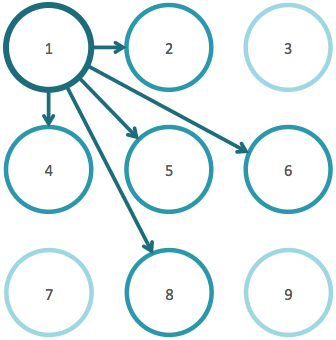
\includegraphics[width=0.4\textwidth]{pics/review/rule1.png}
	      \label{fig:androidrules1}
	    }
	    \hspace{0.8cm}
	    \subfigure[Create a path over a selected node]{
	      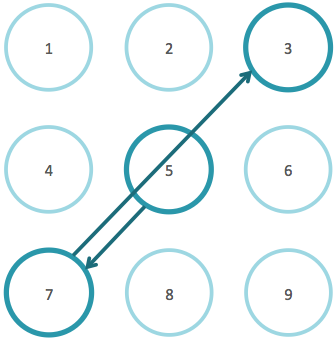
\includegraphics[width=0.4\textwidth]{pics/review/rule2.png}
	      \label{fig:androidrules2}
	    }
	    \caption{Illustration of the Android Pattern creation rules}
	    \label{fig:androidrules}
	  \end{figure}

  In a historical view the Android Unlock pattern is seem as a new authentication mechanism as opposite to alphanumeric passwords and PIN codes. In a security perspective, the pattern has a total of 389,112 possible valid patterns with a $3\times3$ square. Comparing this with PIN codes with a possible number of 10.000 possible codes, the pattern unlock codes seems as a more secure authentication mechanism. Compared to alphanumeric password, it is not a quite higher number of combination, depending on the limit and characters included. When looking at published research, users are normally capable to remember a password with an average length of 7 to 8 characters. As introduced, the Android unlock pattern is a more suitable form of authentication for mobile devices due to its interactive and graphical form that are suitable on small touch screens. When using a alphanumeric password on a small mobile device, you have to use a keyboard that takes more typing the password, making it less suitable for mobile devices. Smartphones are rapidly used in various situation during a day, making it desirable to use a authentication mechanism that is quick to type and easy to remember to avoid spending the time unlocking your smartphone. It is no secret that a alphanumeric password with its extensive password space is more secure, but its not rapidly used on smartphones because of its lack of usability on small devices. To explore the security, usability, and memorability of the Android unlock pattern we will take a look into published research to get a overview.

  	%Table: Number of pattern combinations
	  \begin{table}[H]
	    \centering
	    \begin{tabular}{| l | l |}
	      \hline
	      {\bf \# Length} & {\bf \# Valid combinations} \\ \hline
	      4 & 1624 \\
	      5 & 7152 \\
	      6 & 26,016 \\
	      7 & 72,912 \\
	      8 & 140,704 \\
	      9 & 140,704 \\ \hline
	      Total & 389,112\\ \hline
	    \end{tabular}
	    \caption{Number of pattern combinations}
	    \label{tab:combinations}
	  \end{table}

  As stated, the Andorid pattern lock has a total of 389,112 valid pattern combinations. But is this number as secure as it sounds? When looking at the security of a password scheme it can be looked upon its total combinations (e.g. the password space) or the passwords that statistically users would pick (e.g. the practical password space). In Table \ref{tab:combinations} there is a summary of the total number of valid combinations based on the pattern length \cite{Sun}. An another way to look at security of the patterns is to measure the pattern strength of individual patterns. A published research paper investigate the use of password meter to measure the strength of a pattern. Their hypothesis was that the use of a password meter was providing more secure user selected patterns. They states that there are a high number of valid combinations of patterns, but that users often tend to choose a short and easly guessed pattern due to memorability. A password meter are often shown as a colored bar that is often used as a indication of the strength of a password. The research group used a mathematical equation (\ref{eq:patternstrength}) for calculating the strength of Andorid pattern locks. 

    \begin{equation}\label{eq:patternstrength}
      PS_{P} = S_{P} \times log_{2}(L_{P} + I_{P} + O_{P})
    \end{equation}

  $PS_{p}$ is the strength score of pattern P. $S_{P}$, $L_{P}$, $I_{P}$, and $O_{P}$ are the number of connected nodes, the physical length, the number of intersections, and the number of overlaps of P, respectively. Using Equation \ref{eq:patternstrength} on all valid patterns gives a score from 6.340 to 46.807. The formula was used by Sun et al. \cite{Sun} in their research on Andorid patterns and password meters. They look at pattern strength in a different way then just calculating the complexity of a pattern just by it length. Calculating password complexity by length seems as a naive approach, making this way more realistic using all the rules of the Andorid pattern in the equation. When looking at the different characteristics and strength of a pattern used in Equation \ref{eq:patternstrength}, Sun et al. maked distribution graphs of the different characteristics and the strength (Figure \ref{fig:patterngraph}).

  	%Figure: The distribution of the pattern characteristics and strength
    \begin{figure}[H]
      \centering
      \subfigure[Pattern physical length]{
        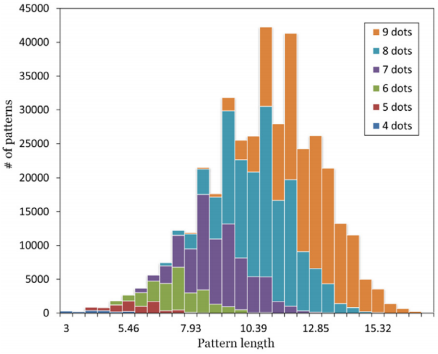
\includegraphics[scale=0.35]{pics/review/patterngraph1}
        \label{fig:patterngraph1}
      }
      \subfigure[Pattern intersections]{
        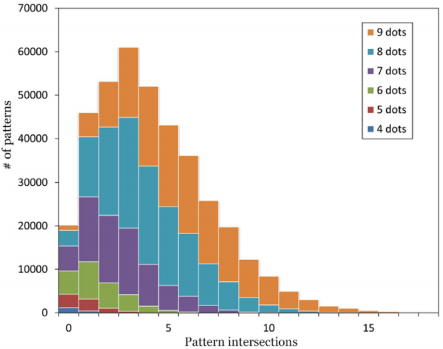
\includegraphics[scale=0.35]{pics/review/patterngraph2}
        \label{fig:patterngraph2}
      }
      \subfigure[Pattern overlaps]{
        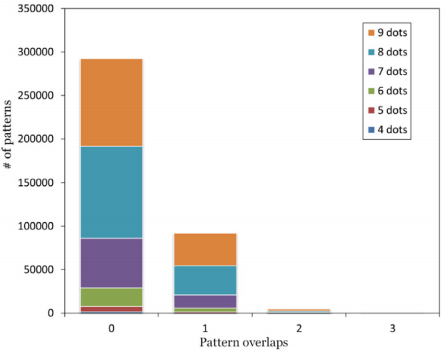
\includegraphics[scale=0.35]{pics/review/patterngraph3}
        \label{fig:patterngraph3}
      }
      \subfigure[Pattern strength]{
        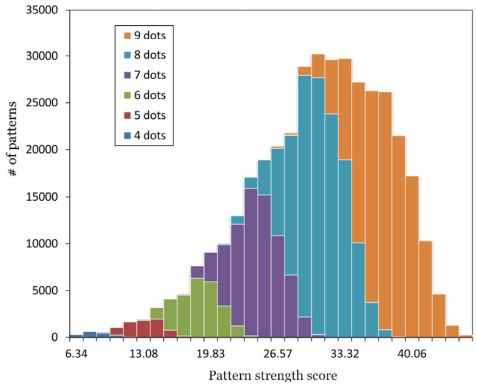
\includegraphics[scale=0.35]{pics/review/patterngraph4}
        \label{fig:patterngraph4}
      }
      \caption{The distribution of the pattern characteristics and strength \cite{Sun}}
      \label{fig:patterngraph}
    \end{figure}

  Sun et al. \cite{Sun} created two different visualizations of a password meter, one looking like a progress bar (Type 1) and one indicating a percent of the strength (Type 2). They recruited a total of 81 participants for a survey testing the strength of user created pattern in three different groups; no password meter (Group A), with password meter type 1 (Group B), and with password meter type 2 (Group C). The survey randomly assigned the participants into the three different groups. The result showed that the strength of patterns in group B and C had a higher complexity and strength, but had a higher error rate when retyping the pattern. As the result showed, users are typically more security conscious when they are aware of the need for such behavior \cite{Sasse}. The error rate shows the problems with passwords and security in general. A long and complex password are harder to guess, but are not likely to be used due to memorability issues. Also a problem with the Android Pattern is that the pattern is rapidly used as it is provided to grant access to the smartphone in all kind of situations. The results from the survey states that the input convince was the reason that caused the highest number of participants in the user study not selecting a pattern with a high complexity and strength. A pattern containing more dots takes longer time to type. When looking at patterns containing intersections and overlaps, there is a higher chance to accidentally hitting the wrong dot when drawing the pattern, causing the user to redraw the pattern and spending more time to passing the authentication. The conclusion is that the time used to type the pattern are as crutial as the time to remember the pattern when looking at the users choice in patterns.

  When looking at user selected passwords, studies shows that many users are using graphical shapes to support memory \cite{Weiss}. Sun et al. \cite{Sun} analyzed the collected patterns and found empirical evidence that some users tended to use patterns which looked like letters or numbers. They found patterns looking like the letters and numbers C, L, N, Z, 2, and 7 that easily can be created on a 3$\times$3 grid. Such a memorability strategy are using association elements, e.g something that the user are familiar with, to increase the memorability. Same strategy are known in PIN codes and alphanumeric passwords where names, objects, dates are used to remember the password.

  One of the traditional password schemes on smartphones is the Android Unlock pattern. It is a graphical password scheme that have been shown to have biases when the password is user-chosen. A research group did one of the first large-scale user study on the security of the Android Unlock Patterns in order to quantify its security \cite{Uellenbeck}. They analyze the biases introduced in the pattern making process and added changes to the scheme in order to avoid the known biases in the password scheme. The researchers found that there is a high bias in the pattern selection process, e.g. the upper left corner and three-point long straight lines are very typical selection strategies. If the patterns were uniformly chosen, the probability of starting in at any point should be 11\%. The results showed that there was a strong bias to the starting point towards the corners. If the points were uniformly chosen, the probability for all four corners should be 44\%, but the results showed that the probability is close to 75\% in the pen-and-paper study. In contrast to this, the center point, the right, the upper, and the lower center points only get a probability of 14\% based on the results. Other results from the pen-and-paper study found that the average pattern length was 5.63 (with a standard deviation of 1.5). By looking further into the pattern length chosen by users, this is not a surprisingly result because this seems quite familiar with restriction of the Android Pattern Lock that requires the users to make a pattern of at least 4 connected points. As stated earlier, users tend to take the easiest way out, making users choose short patterns that are easy to remember and type. Besides the pen-and-paper study, there was also conducted a user study that also showed a high bias towards the upper-left corner that had the bias of 43\% in the user study, and 38\% in the pen-and-paper study. This is supporting the researchers claim that users tend to choose less secure patterns ``in the wild''.

  \clearpage

    \begin{figure}[H]
      \centering
      \vspace{1.5cm}
      \subfigure[Sequence: 147852369, \newline Strength: 27.00]{
        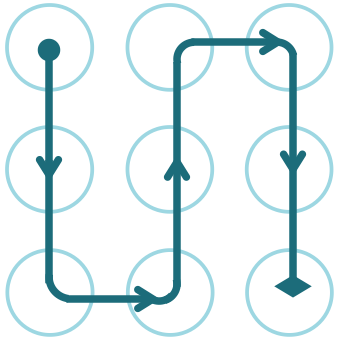
\includegraphics[width=0.27\textwidth]{pics/experiment/strengthpattern2.png}
        \hspace{0.6cm}
      }
      \subfigure[Sequence:213546879, \newline Strength: 36.655]{
        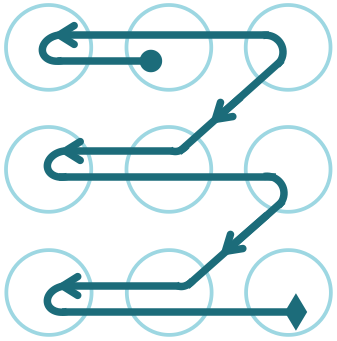
\includegraphics[width=0.27\textwidth]{pics/experiment/strengthpattern3.png}
        \hspace{0.6cm}
      }
      \subfigure[Sequence: 591827346, \newline Strength: 46.807]{
        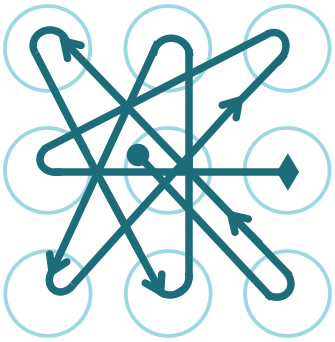
\includegraphics[width=0.27\textwidth]{pics/experiment/strengthpattern1.png}
      }
      \vspace{0.5cm}

      \subfigure[Sequence: 968752, \newline Strength: 15.259]{
        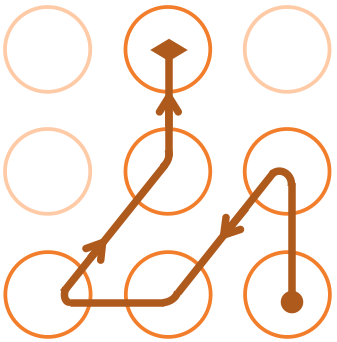
\includegraphics[width=0.27\textwidth]{pics/experiment/strengthpattern7.png}
        \hspace{0.6cm}
      }
      \subfigure[Sequence: 1269853, \newline Strength: 20.781]{
        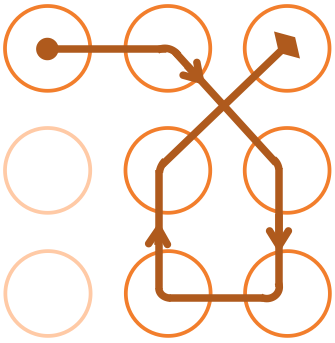
\includegraphics[width=0.27\textwidth]{pics/experiment/strengthpattern8.png}
        \hspace{0.6cm}
      }
      \subfigure[Sequence: 36578249, \newline Strength: 30.512]{
        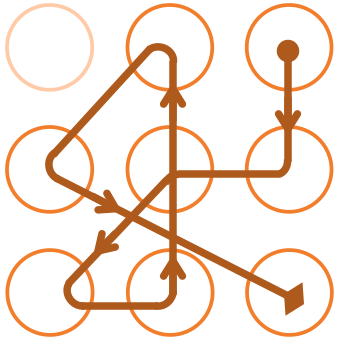
\includegraphics[width=0.27\textwidth]{pics/experiment/strengthpattern9.png}
      }
      
      \vspace{0.5cm}

      \subfigure[Sequence: 1478, \newline Strength: 6.339]{
        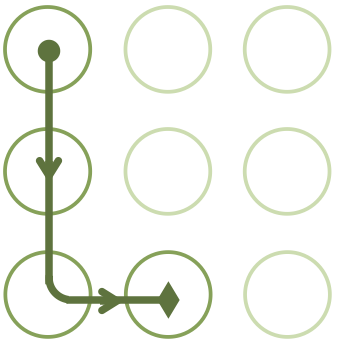
\includegraphics[width=0.27\textwidth]{pics/experiment/strengthpattern4.png}
        \hspace{0.6cm}
      }
      \subfigure[Sequence: 5968, \newline Strength: 9.086]{
        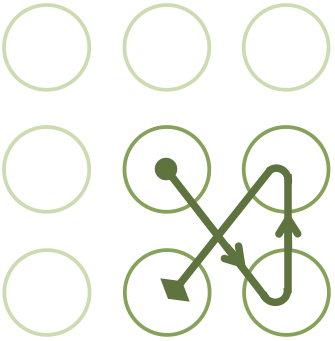
\includegraphics[width=0.27\textwidth]{pics/experiment/strengthpattern5.png}
        \hspace{0.6cm}
      }
      \subfigure[Sequence: 4927, \newline Strength: 11.786]{
        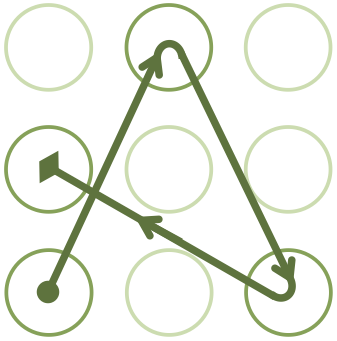
\includegraphics[width=0.27\textwidth]{pics/experiment/strengthpattern6.png}
      }

      \vspace{0.5cm}
      \caption{Examples of patterns with different length and strength}
    \end{figure}

    \todo[inline, color=blue!60]{Må her vise til disse forskjellige mønstrene som viser hvordan styrken defineres. Refereres til i tekst.}
